\lecture{Bivariate Data}{bivariate-data}
\section{Bivariate Data}

\title{Bivariate data}
\subtitle{Determining Relationships From Two Related Data Sets}

%\author{Kelly Black}
%\institute{Clarkson University}
\date{17 November 2014}

\begin{frame}
  \titlepage
\end{frame}

\begin{frame}
  \frametitle{Outline}
  \tableofcontents[hideothersubsections,sectionstyle=show/hide]
\end{frame}



\subsection{Clicker Quiz}

\begin{frame}{Clicker Quiz}

  \iftoggle{clicker}{%

    Suppose that \\
    \begin{tabular}{r@{~$=$~}l}
      $x$ & Age of Cat (between 0 and 1 year)  \\
      $y$ & Mass of Cat (kg)
    \end{tabular}

    \vfill

    If $x$ increases what do you expect to happen to $y$?

    \vfill 


    \begin{tabular}{l@{\hspace{3em}}l@{\hspace{3em}}l@{\hspace{3em}}l}
      A: $y$ tends to inc.  & B: No trend & C: $y$ tends to dec.
    \end{tabular}

    \vfill
    \vfill
    \vfill

  }

\end{frame}

\subsection{Bivariate Data}




\begin{frame}
  \frametitle{Define the terms}

  \begin{columns}
    \column{.25\textwidth}

    \begin{tabular}{l|l}
      $X$ & $Y$ \\ \hline
      $x_1$ & $y_1$ \\
      $x_2$ & $y_2$ \\
      $x_3$ & $y_3$ \\
      $x_4$ & $y_4$ \\
      $\vdots$ & $\vdots$ \\
      $x_n$ & $y_n$ \\
    \end{tabular}


    \vfill

    \column{.75\textwidth}

    \only<2->
    {
      There is a ``one to one'' correspondence between each
      row. i.e. $x_3$ and $y_3$ are related to one another.

    }

    \vfill

  \end{columns}


  \begin{columns}
    \column{.5\textwidth}

    \only<3-> {

      Examine $x$ by itself: \\
      \begin{tabular}{l}
        N \\
        $\bar{x}$ \\
        $s_x$
      \end{tabular}

      Standard statistics.

    }
      
    \column{.5\textwidth}


    \only<4-> {

      Examine $y$ by itself: \\
      \begin{tabular}{l}
        N \\
        $\bar{y}$ \\
        $s_y$
      \end{tabular}

      Standard statistics.


    }


  \end{columns}


\end{frame}



\begin{frame}
  \frametitle{Bivariate Data}

  \textbf{After} the uni-variate statistics for the $x_i$ and the
  $y_i$ data is examined then you can bring them together and explore
  the \textit{relationship}:
  \begin{eqnarray*}
    \begin{array}{l|l}
      X & Y \\ \hline
      x_1 & y_1 \\
      x_2 & y_2 \\
      x_3 & y_3 \\
      x_4 & y_4 \\
      \vdots & \vdots \\
      x_n & y_n
  \end{array}
\end{eqnarray*}

\end{frame}

\begin{frame}
  \frametitle{Example}

  \begin{columns}
    \column{.25\textwidth}

  \begin{eqnarray*}
    \begin{array}{r|r}
      X & Y \\ \hline
      3 & 6 \\
      2 & 2 \\
      -1 & -3 \\
      4 & 4 \\
      2 & 3
    \end{array}
  \end{eqnarray*}


    \column{.75\textwidth}

  \only<4->
  {
    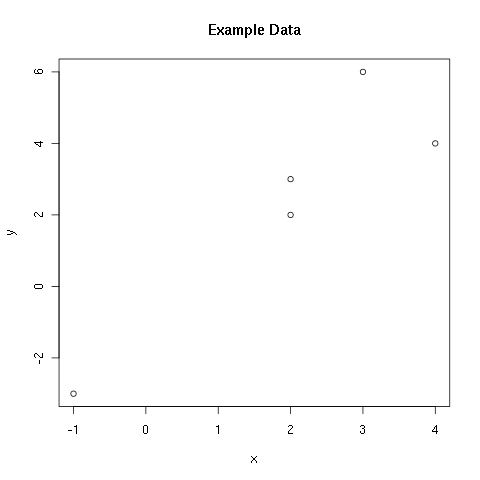
\includegraphics[width=5cm]{img/simpleBivariateExample}
  }


  \end{columns}

  \begin{columns}
    \column{.5\textwidth}

    \only<2-> {

      Examine $x$ by itself: \\
      \begin{tabular}{lllll}
        \multicolumn{5}{l}{$N=5$} \\
        \multicolumn{5}{l}{$\bar{x}=2.00$} \\
        \multicolumn{5}{l}{$s_x=1.871$} \\
        Min & Q1 & Med & Q3 & Max \\
        -1.0 & 2.0 & 2.0 & 3.0 & 4.0
      \end{tabular}


    }
      
    \column{.5\textwidth}


    \only<3-> {

      Examine $y$ by itself: \\
      \begin{tabular}{lllll}
        \multicolumn{5}{l}{$N=5$} \\
        \multicolumn{5}{l}{$\bar{y}=2.40$} \\
        \multicolumn{5}{l}{$s_y=3.362$} \\
        Min & Q1 & Med & Q3 & Max \\
        -3.0 & 2.0 & 3.0 & 4.0 & 6.0
      \end{tabular}



    }


  \end{columns}


\end{frame}



\begin{frame}{Now Bring Them Together}

  Graphically, we can look at the scatter plot:

  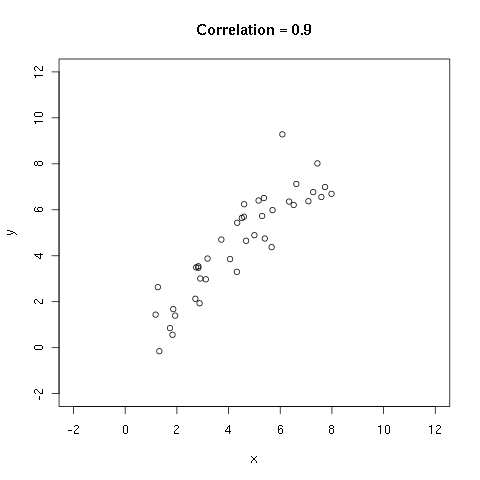
\includegraphics[height=4cm]{img/correlation09}
  
\end{frame}



\begin{frame}{Positive vs. Negative Relationships}

  \begin{columns}
    \column{.45\textwidth}

    \begin{definition}
      If $y$ \textbf{tends} to increase as $x$ increases then we say
      that it is a \textit{positive relationship} : \\
      \centerline{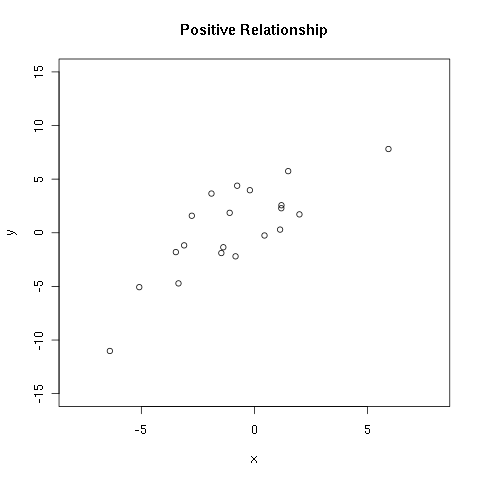
\includegraphics[width=5cm]{img/positiveRelationship}}
    \end{definition}

    \column{.5\textwidth}

    \begin{definition}
      If $y$ \textbf{tends} to decrease as $x$ increases then we say
      that it is a \textit{negative relationship} : \\
      \centerline{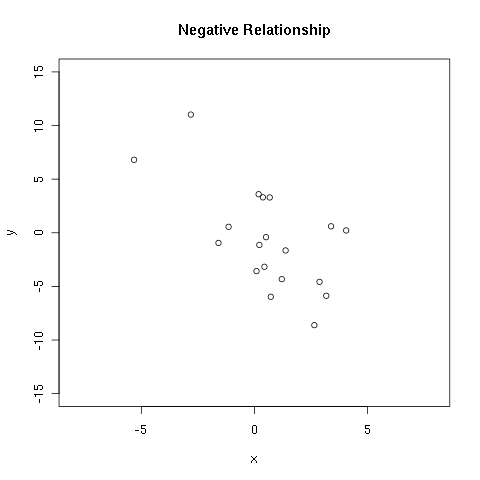
\includegraphics[width=5cm]{img/negativeRelationship}}
    \end{definition}

  \end{columns}
  
\end{frame}


\begin{frame}{Clicker Quiz}

  \iftoggle{clicker}{%

    Suppose that \\
    \begin{tabular}{r@{~$=$~}l}
      $x$ & Age of Cat (between 0 and 1 year)  \\
      $y$ & Mass of Cat (kg)
    \end{tabular}

    \vfill

    Is this is a positive or negative relationship?

    \vfill 


    \begin{tabular}{l@{\hspace{3em}}l@{\hspace{3em}}l@{\hspace{3em}}l}
      A: Positive  & B: Negative
    \end{tabular}

    \vfill
    \vfill
    \vfill

  }

\end{frame}


\begin{frame}{Linear Regression}

  Given data can I find the ``best'' straight line
  \begin{eqnarray*}
    y & = & \beta_0 + \beta_1 x?
  \end{eqnarray*}


  \only<1>{\centerline{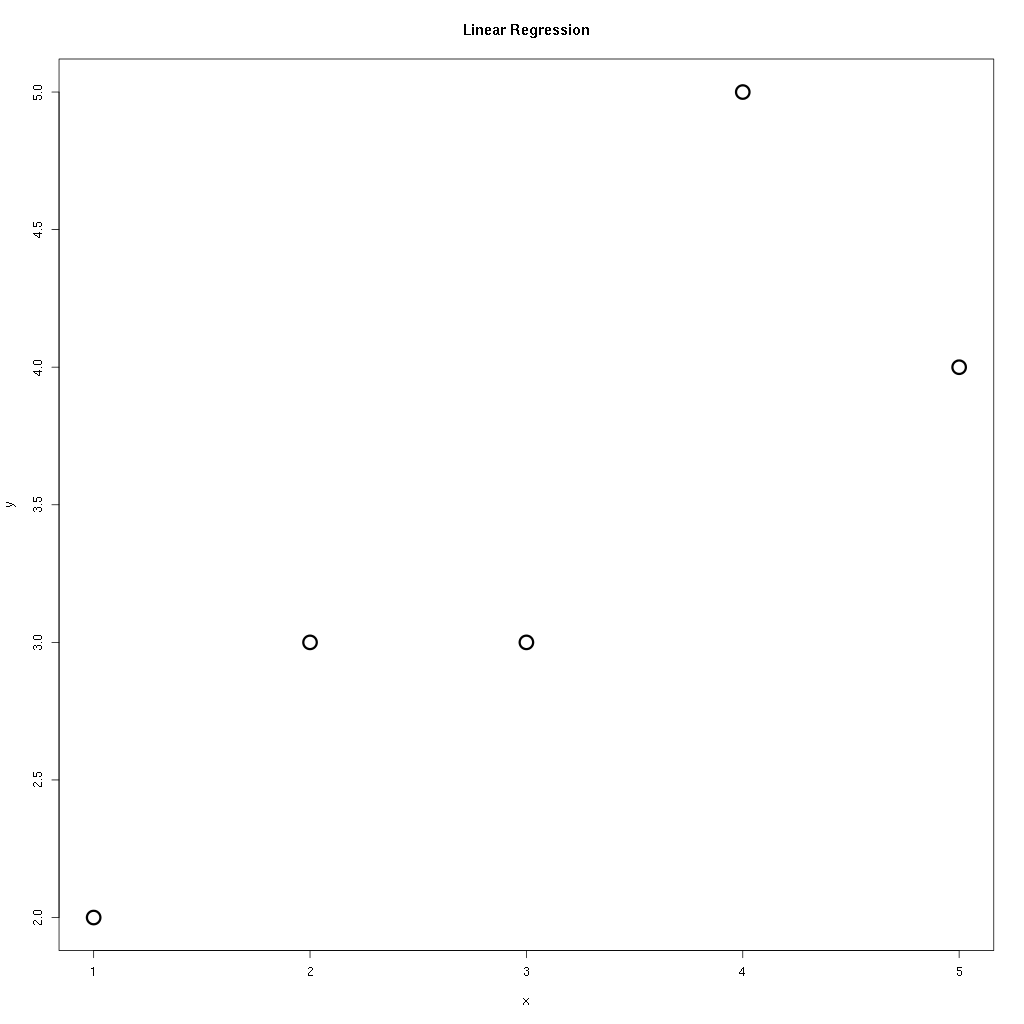
\includegraphics[width=4cm]{img/scatterLR-raw}}}
  \only<2>{\centerline{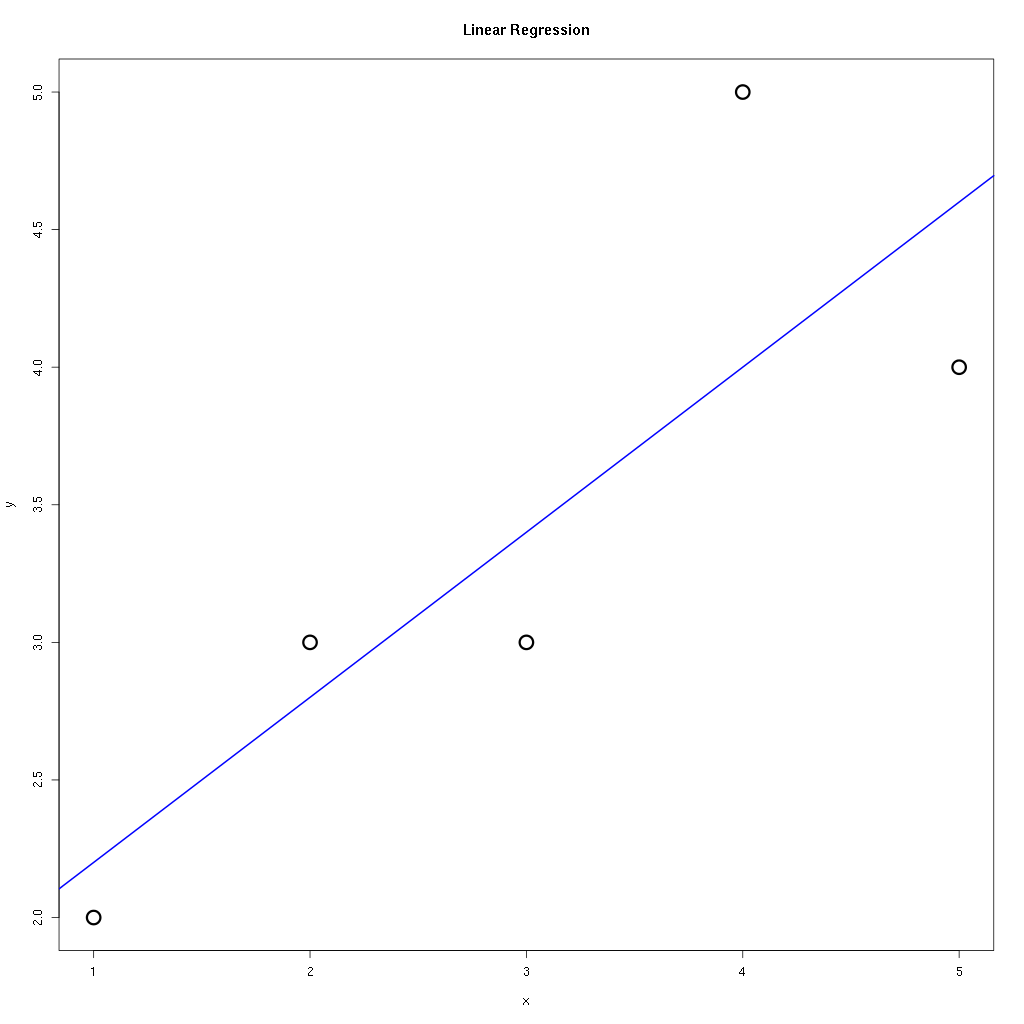
\includegraphics[width=4cm]{img/scatterLR-line}}}
  
\end{frame}


\begin{frame}{Linear Model}

  We model a linear relationship:
  \only<1>{%
    \begin{eqnarray*}
      y_i & = & \beta_0 + \beta_1 x_i + \epsilon_i.
    \end{eqnarray*}
  }
  \only<2->{%
    \begin{eqnarray*}
      y_i & = & \redText{\beta_0 + \beta_1 x_i} + \blueText{\epsilon_i},
    \end{eqnarray*}
    \begin{itemize}
    \item \redText{Straight line relationship: $\beta_0 + \beta_1 x$,}
    \item \blueText{Error: $\epsilon_i$.}
    \end{itemize}
  }
  \only<3->{%

    Assumptions:
    \begin{itemize}
    \item The error is normally distributed with mean zero and
      variance $\sigma^2$.
    \item The value of $x_i$ is known to a higher level of certainty. 
    \end{itemize}

  }
  
\end{frame}

\begin{frame}{The Distribution of Y}

  \begin{block}{Distribution of Y}
    The random variable $y_i$ is a normally distributed random
    variable with mean $\beta_0+\beta_1x_i$.
  \end{block}

    \only<2>{%
      \centerline{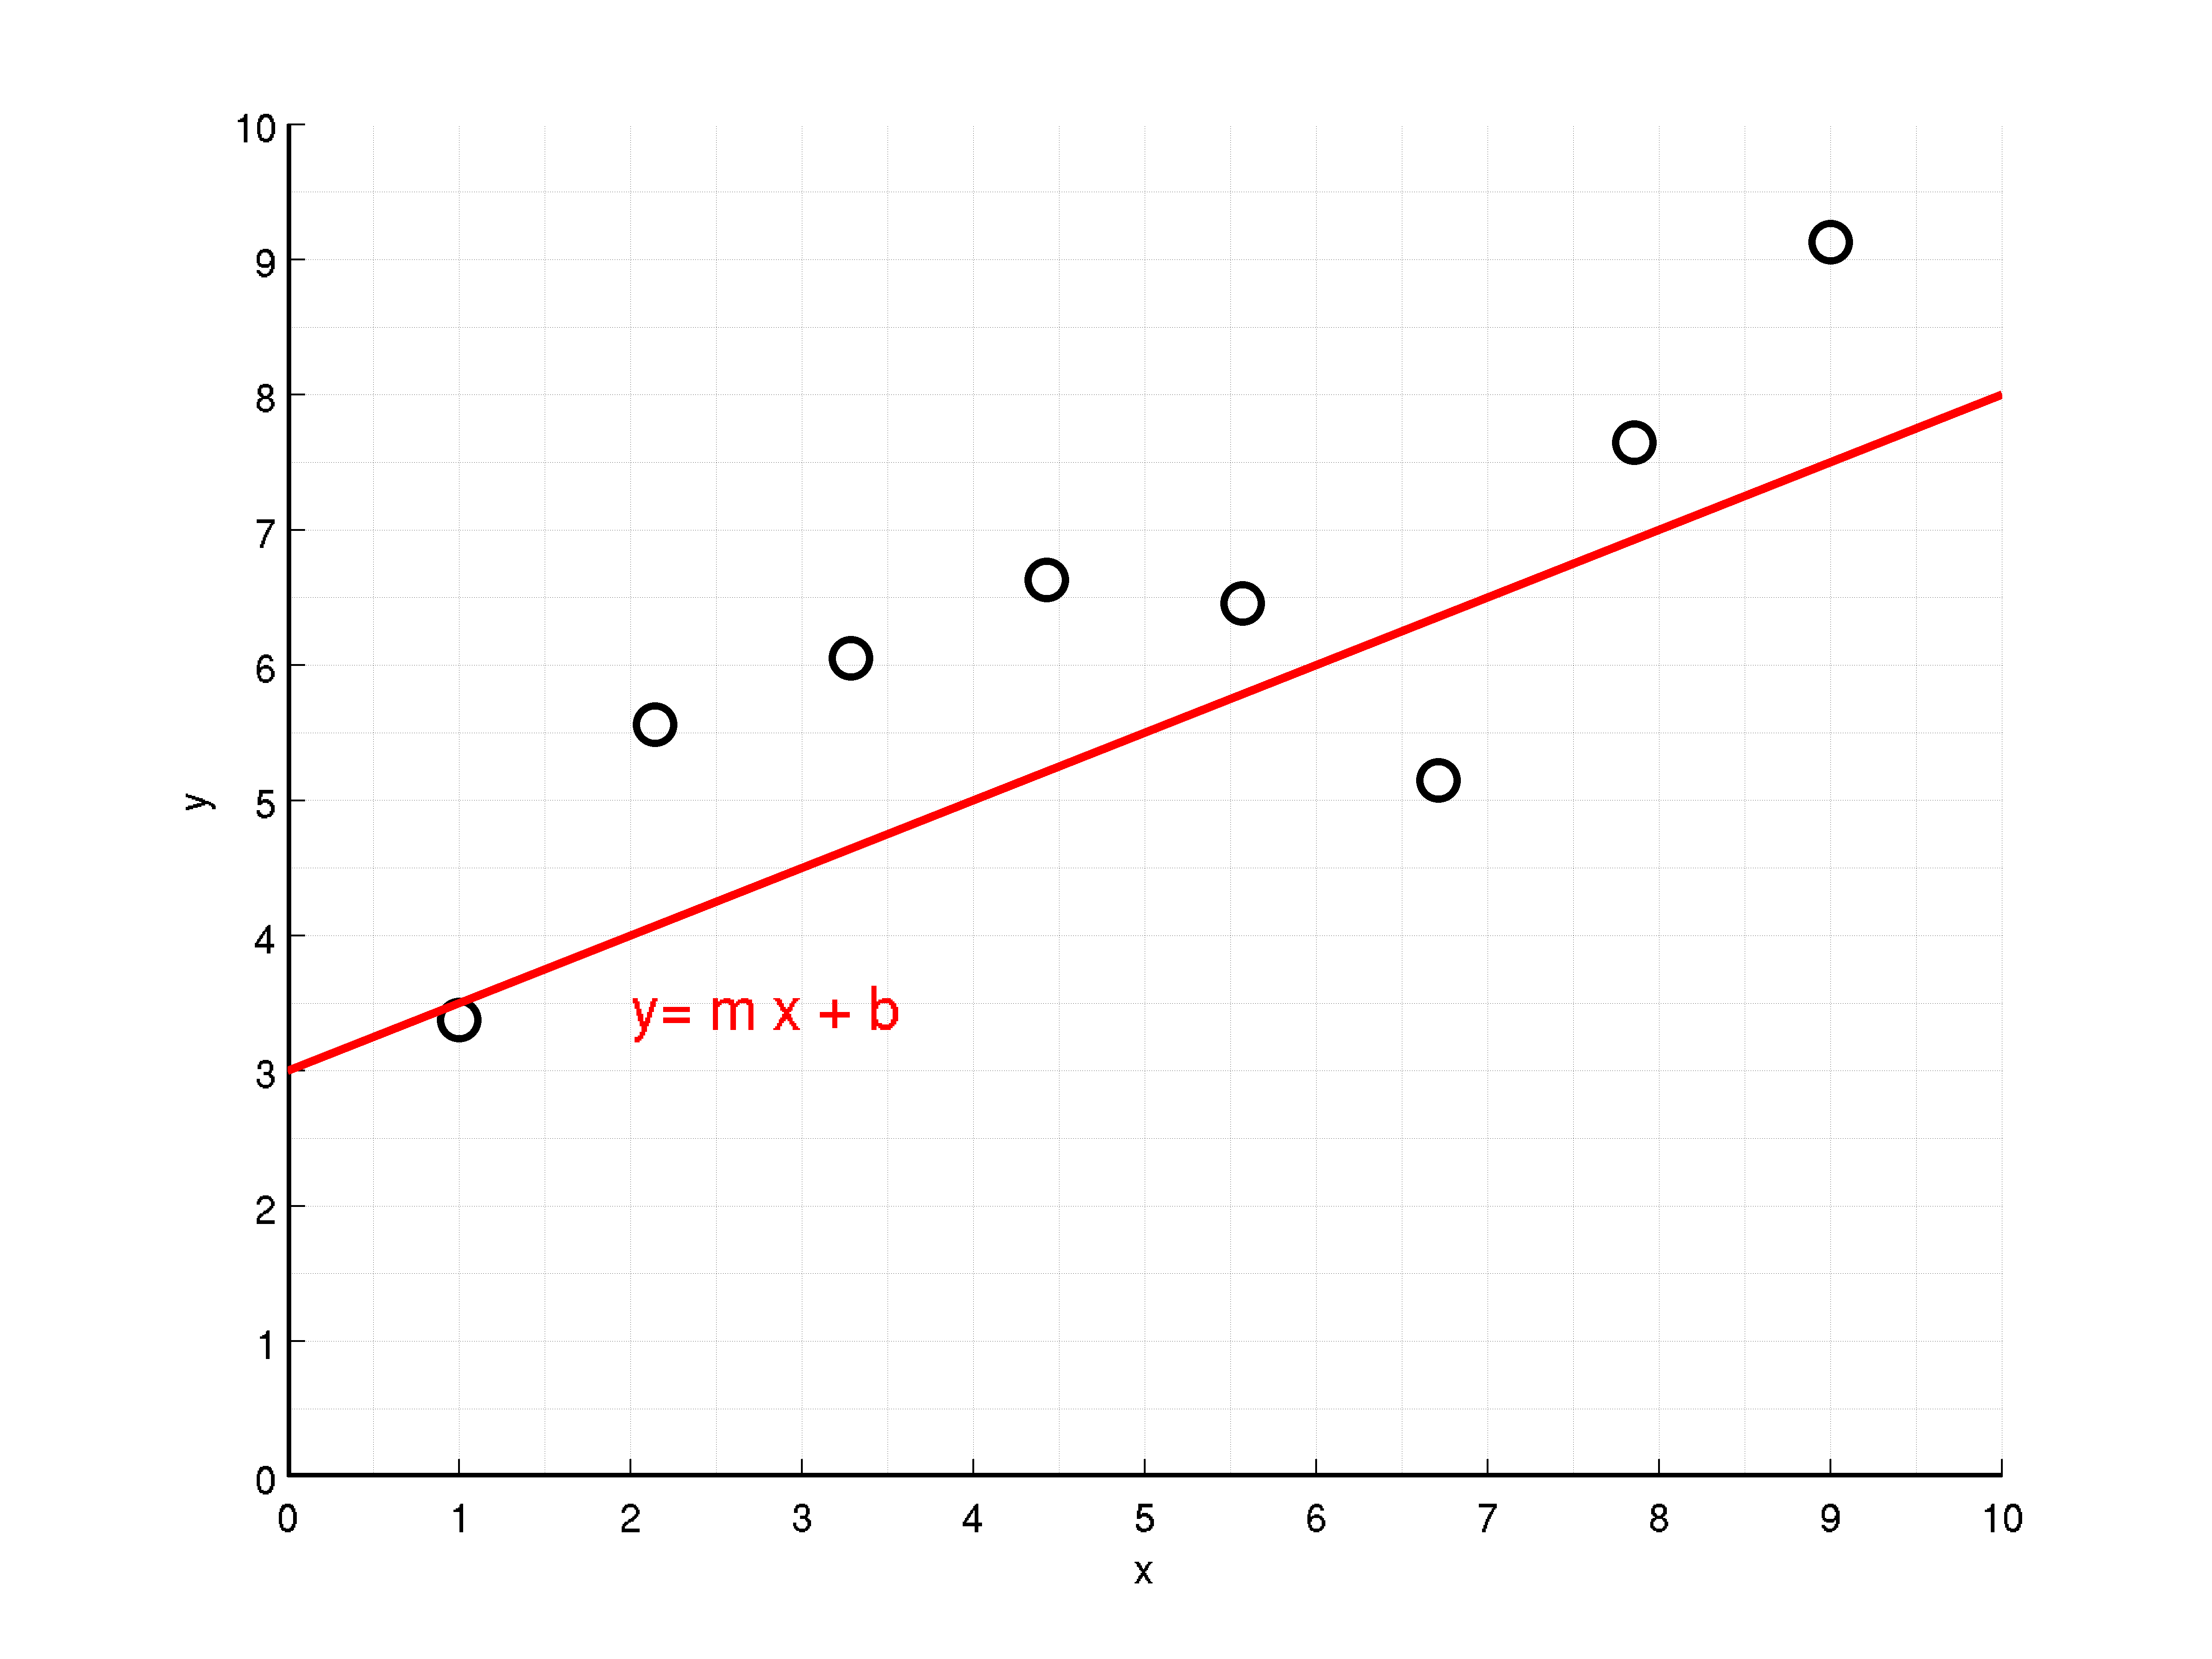
\includegraphics[width=5cm]{img/regressionInferenceOne}}
    }

    \only<3>{%
      \centerline{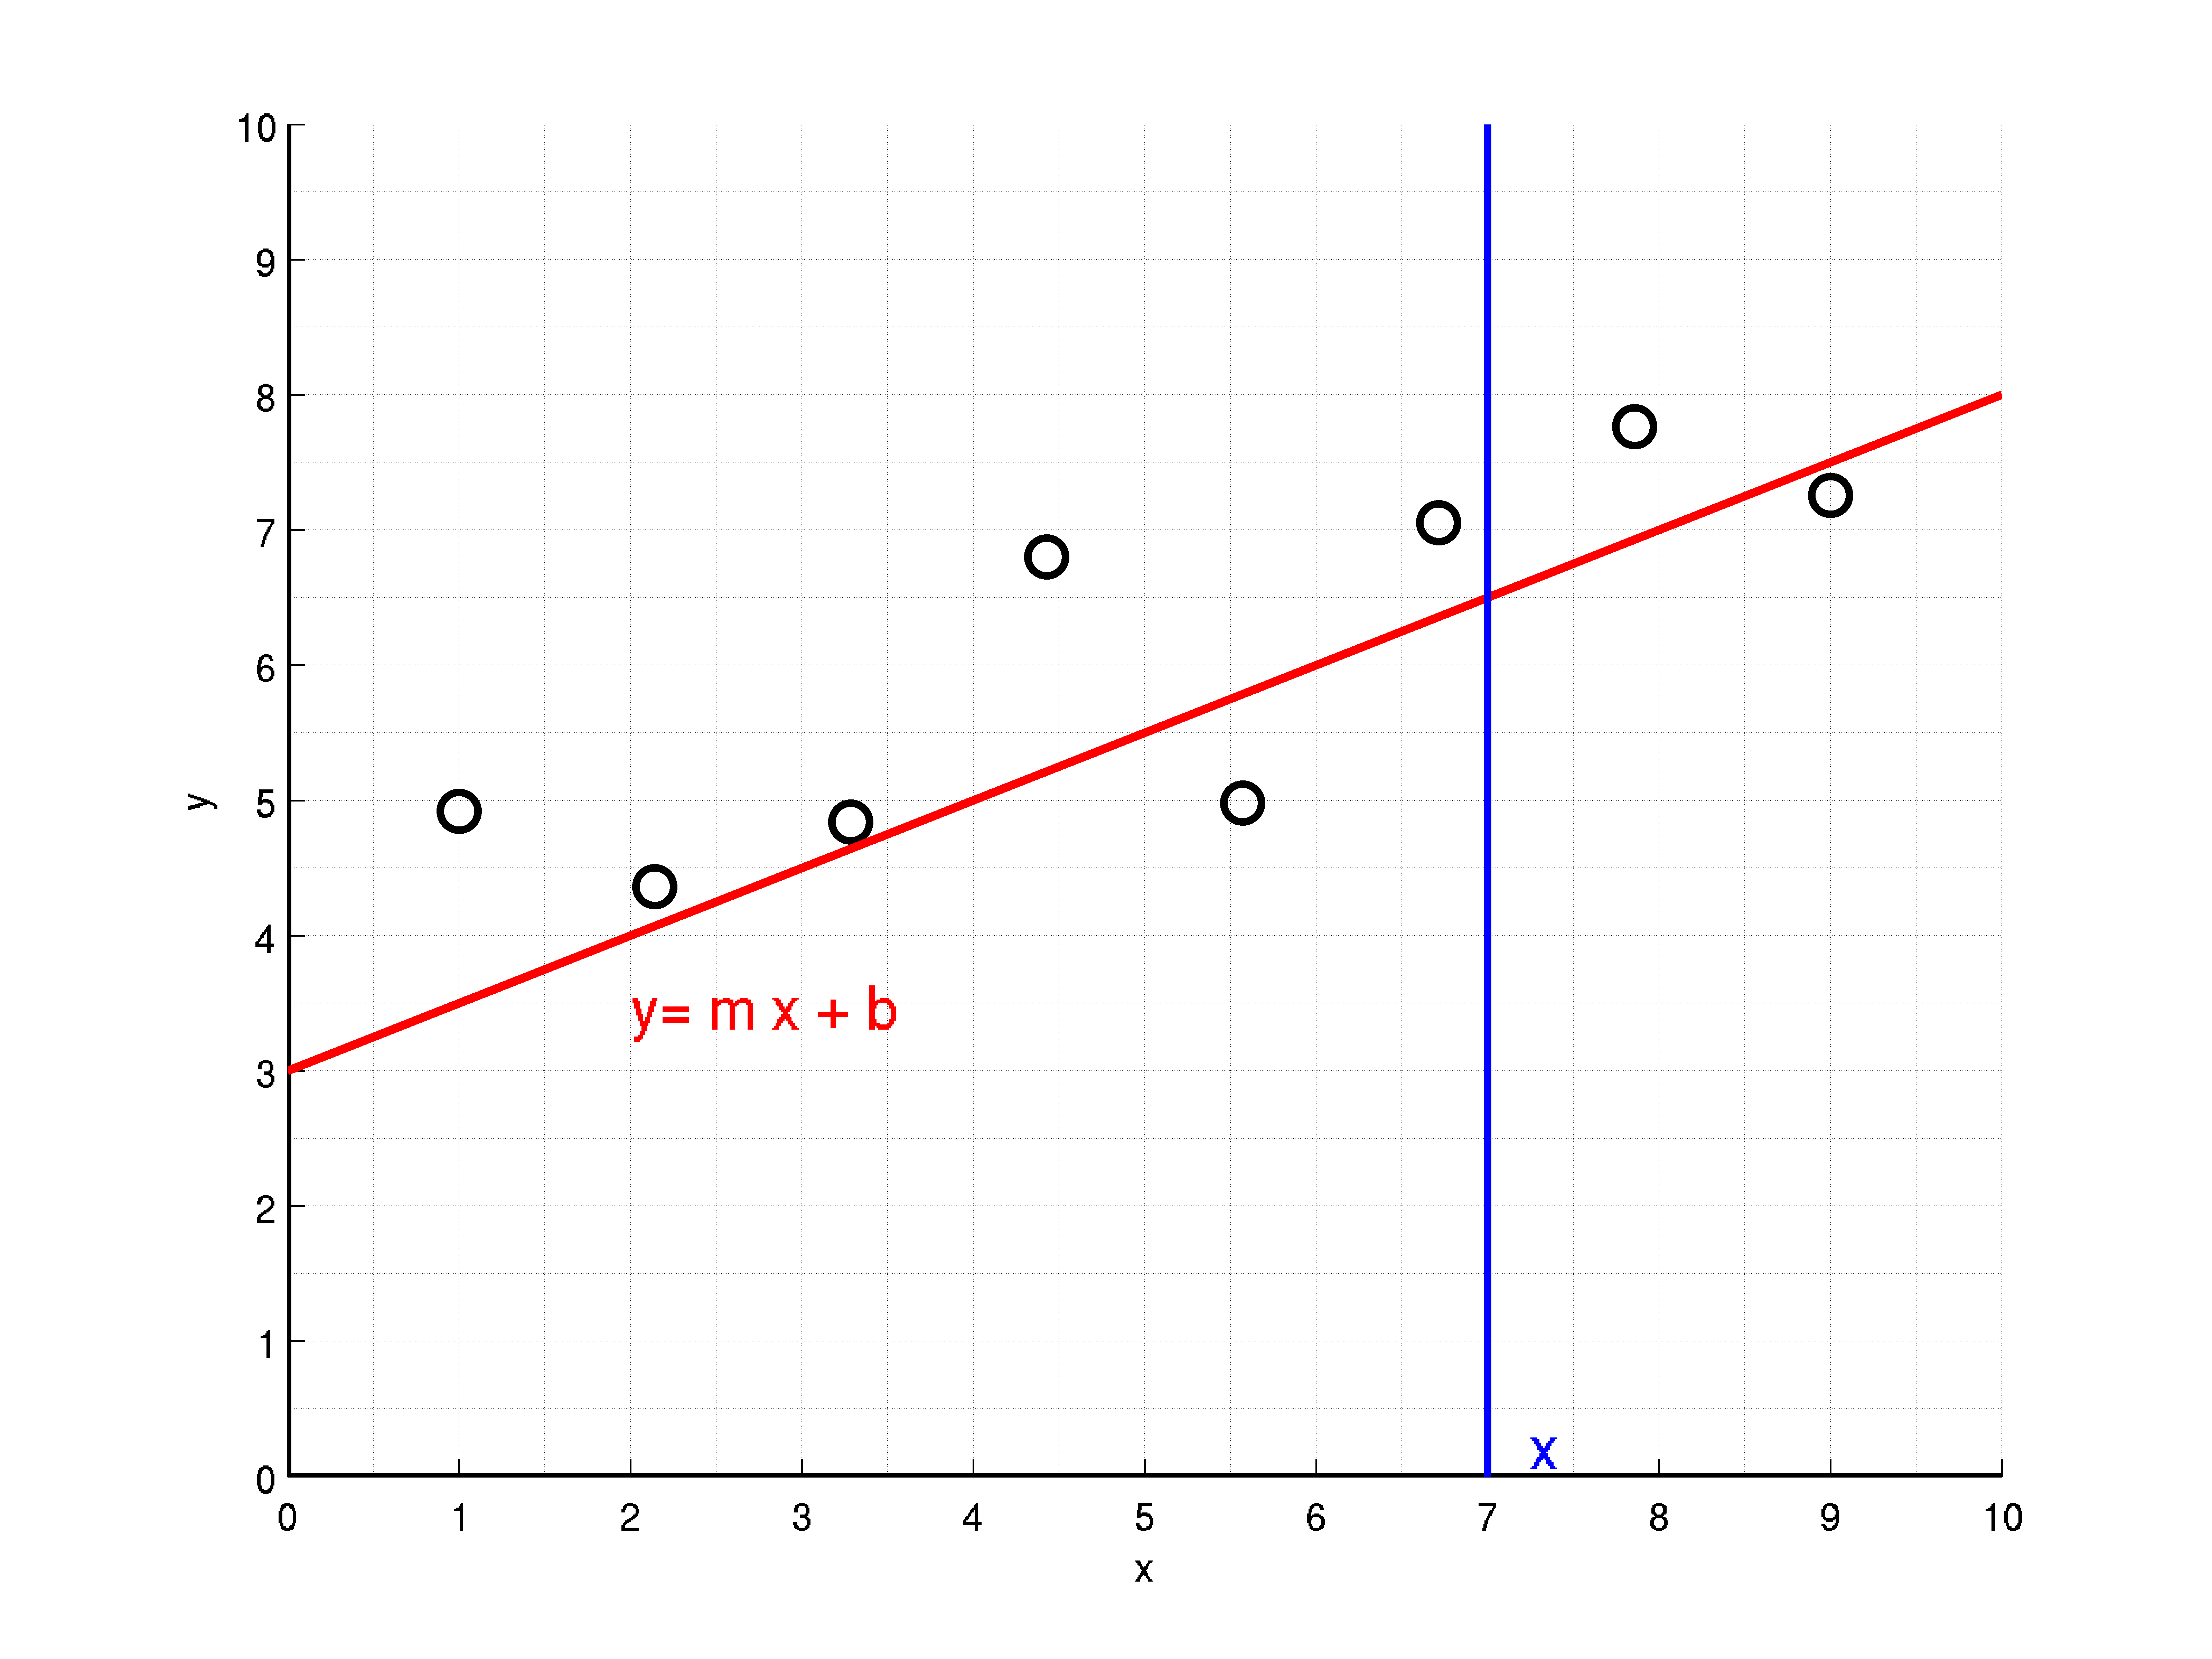
\includegraphics[width=5cm]{img/regressionInferenceTwo}}
    }

    \only<4>{%
      \centerline{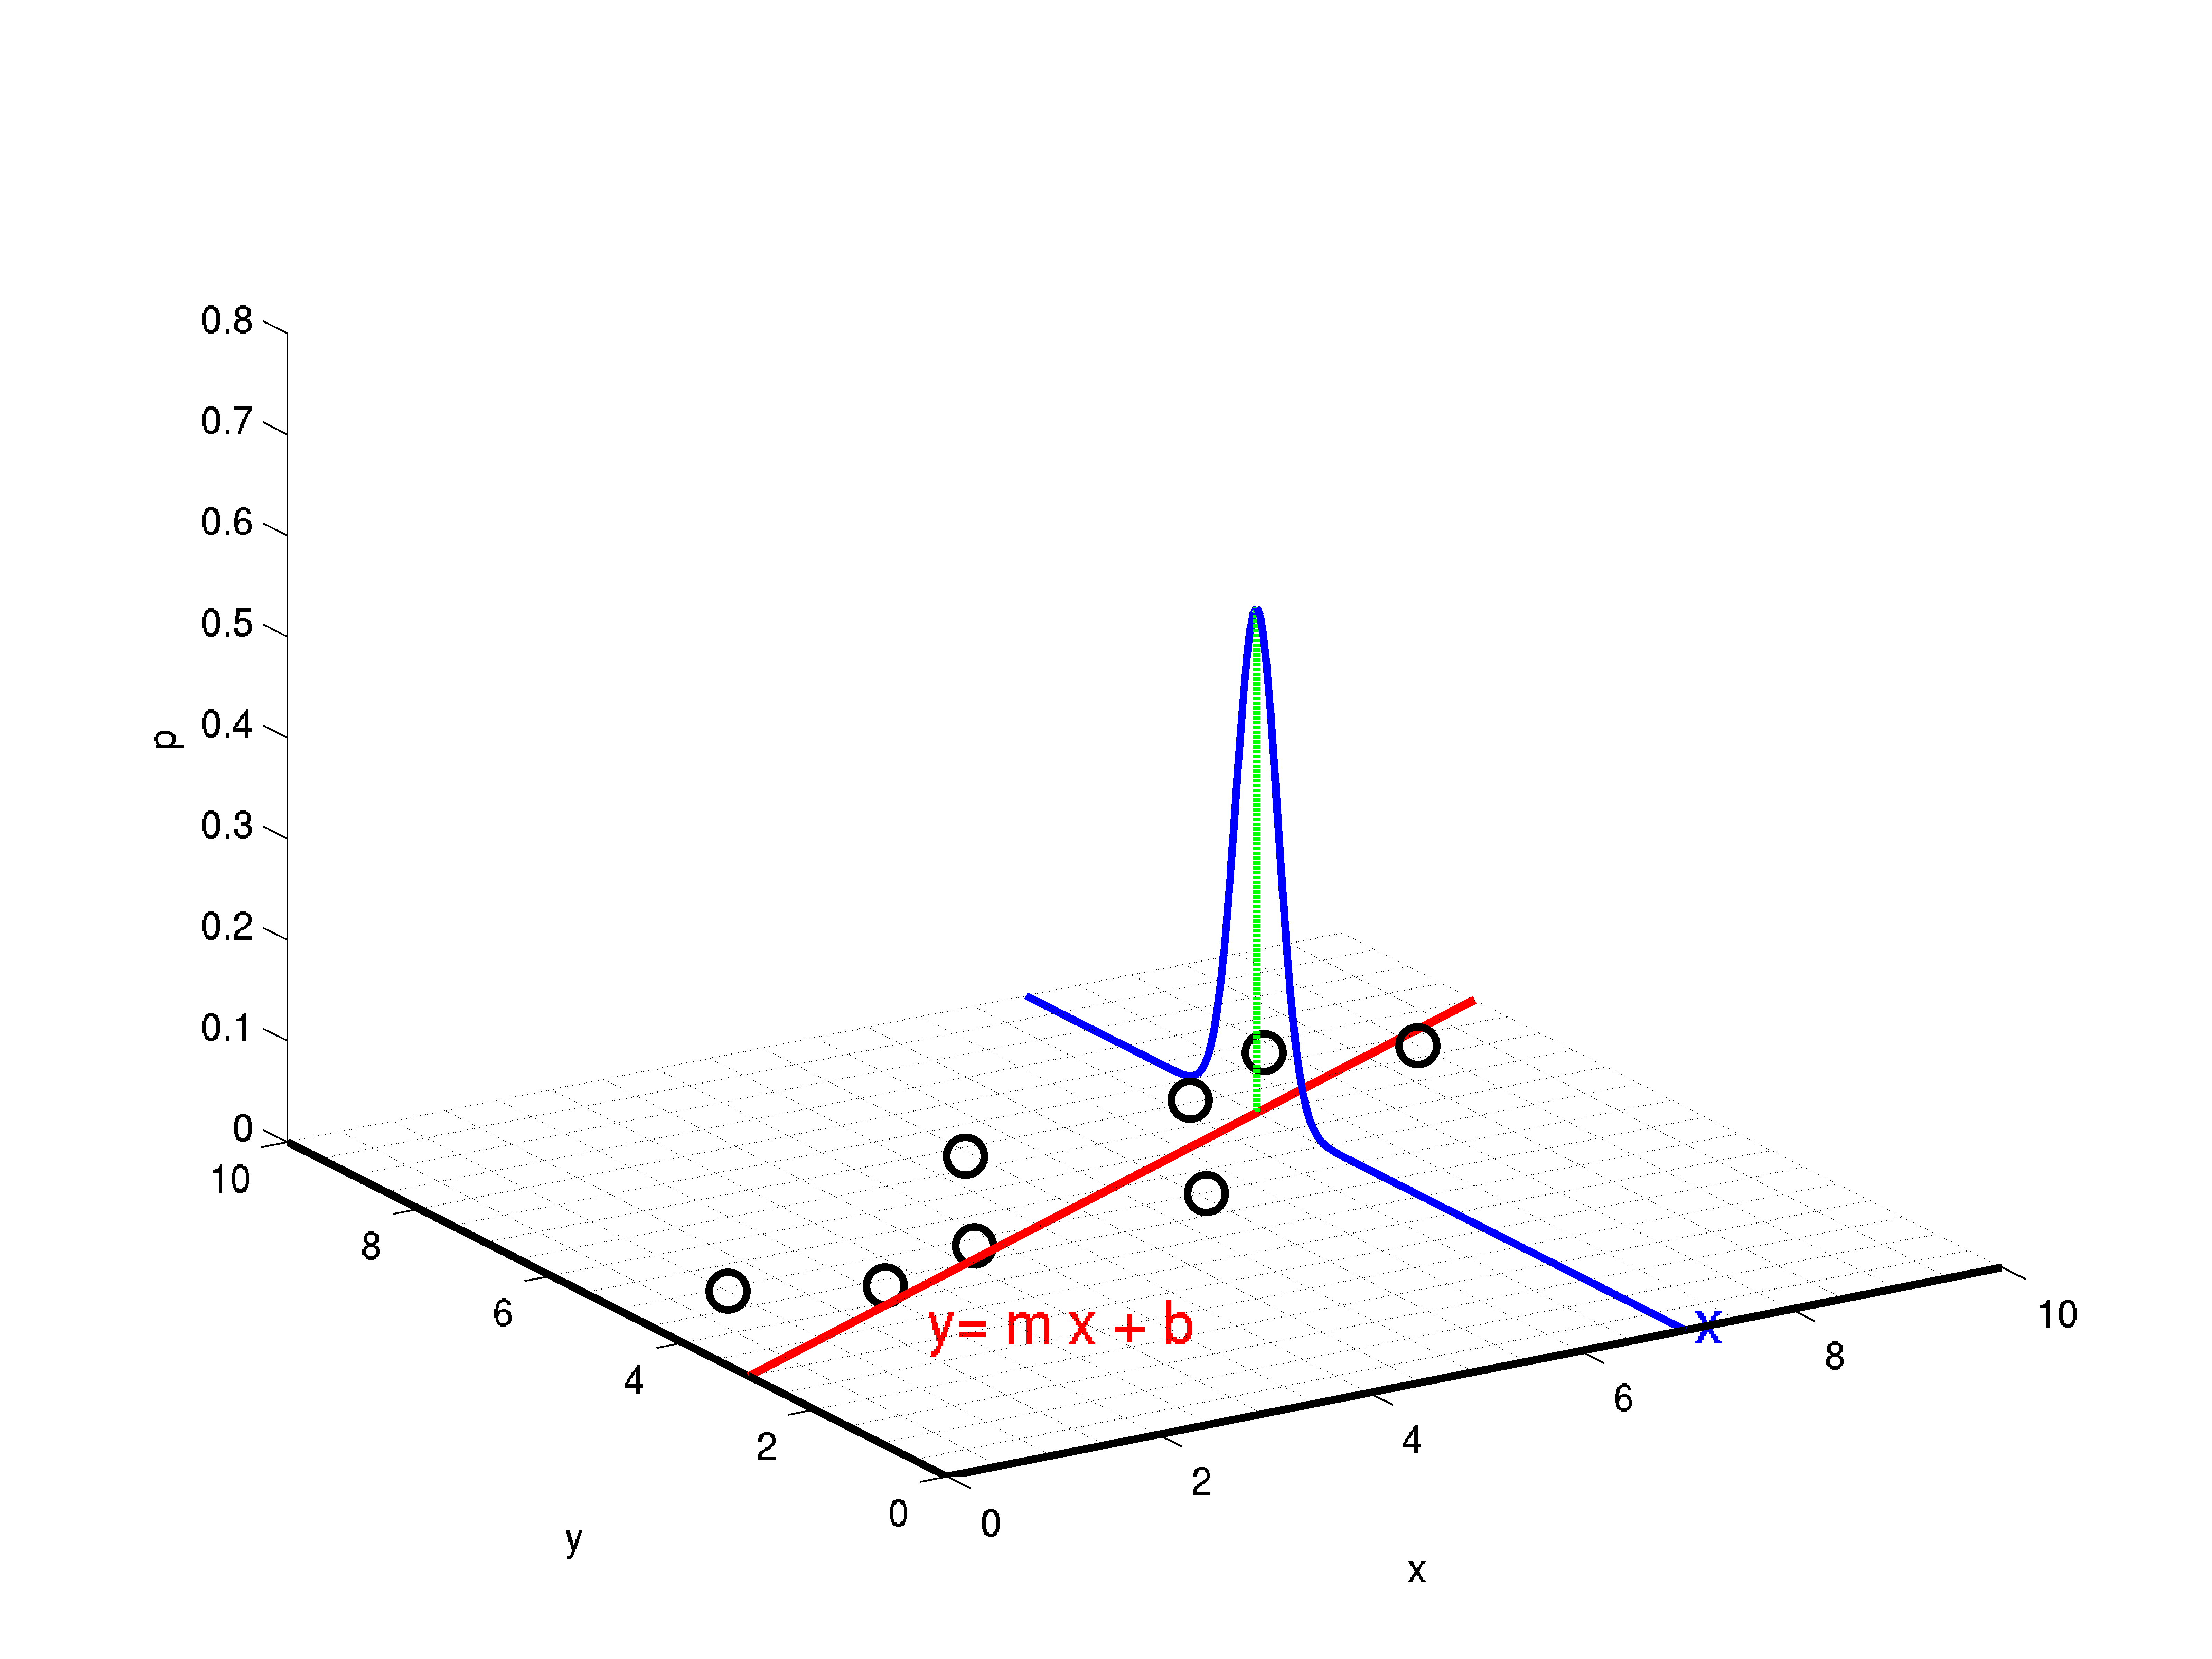
\includegraphics[width=5cm]{img/regressionInferenceThree}}
    }

  
\end{frame}

\begin{frame}{Question}
  
  \begin{columns}
    \column{.25\textwidth}

    \begin{tabular}{l|l}
      $X$ & $Y$ \\ \hline
      $x_1$ & $y_1$ \\
      $x_2$ & $y_2$ \\
      $x_3$ & $y_3$ \\
      $x_4$ & $y_4$ \\
      $\vdots$ & $\vdots$ \\
      $x_n$ & $y_n$ \\
    \end{tabular}


    \vfill

    \column{.75\textwidth}

    Given the data can we estimate $\beta_0$, $\beta_1$, and $\sigma^2$.

    \vfill

  \end{columns}

\end{frame}

\begin{frame}{Example}

  \begin{columns}
    \column{.25\textwidth}

    Flow rate for Aswan Dam 
    \begin{tabular}{l|l|l}
      Year & Jan & Feb \\ \hline
      1874 & 6.4 & 4.4\\
      1875 & 4.1 & 2.4\\
      1876 & 5.4 & 4.1\\
      1877 & 3.3 & 1.8 \\
      $\vdots$ & $\vdots$ & $\vdots$\\
      1984 & 3.7 & 2.8 \\
      1985 & 3.9 & 2.8 \\
      1986 & 3.5 & 2.9 \\
      1987 & 3.8 & 4.0 \\
      1988 & 3.7 & 3.1
    \end{tabular}


    \vfill

    \column{.75\textwidth}

    {\tiny
      Summary:\\
      \begin{tabular}{llllll}
        Min. & 1st Qu.  & Median     & Mean & 3rd Qu. &   Max.  \\
        Jan \\
        1.640 &  3.345 &  3.850 &  4.025 &  4.625 &  7.070  \\
        Feb. \\
        1.230 &  2.170 &  2.850 &  2.896 &  3.435 &  5.670 \\
      \end{tabular}
    }

    \hfill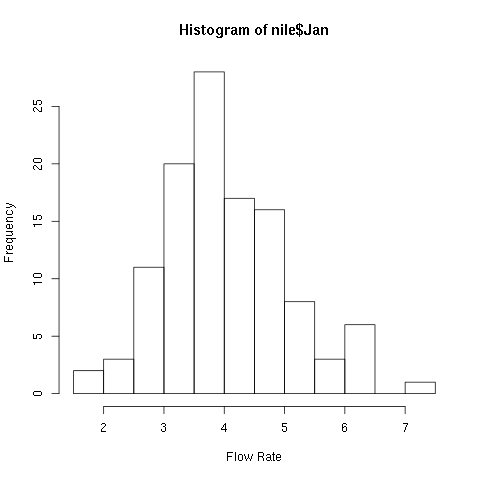
\includegraphics[height=3cm]{img/aswanJan}

    \hfill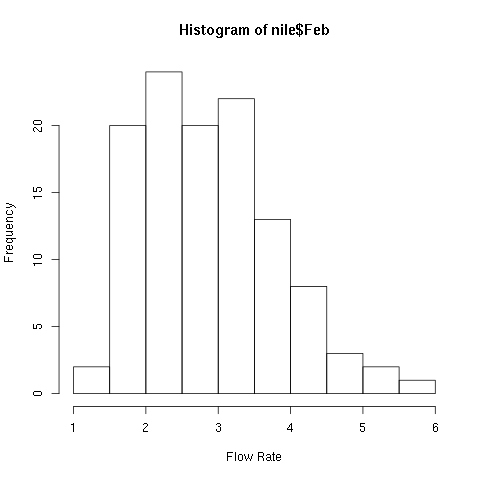
\includegraphics[height=3cm]{img/aswanFeb}

    \vfill

  \end{columns}
  
\end{frame}

\begin{frame}{Aswan Dam as Bivariate Data}

  \only<1>{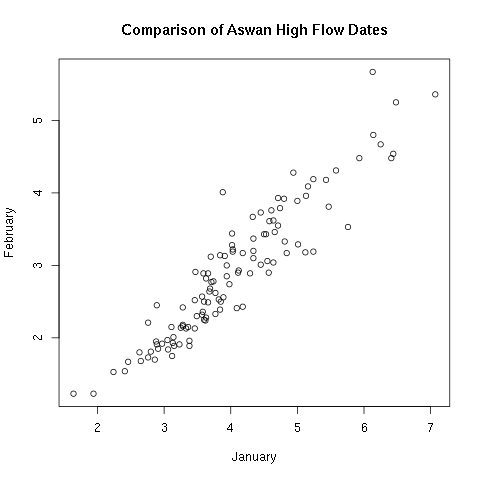
\includegraphics[height=6cm]{img/aswanBivariate}}

  \only<2>{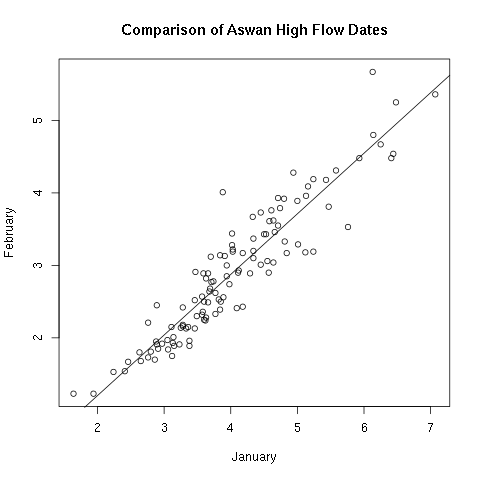
\includegraphics[height=6cm]{img/aswanBivariateRegression}}
  
\end{frame}

\begin{frame}[fragile]
  \frametitle{R Commands}

{\tiny
\begin{verbatim}
  # Read the data
  nile = read.csv(file="fig12.8-nile-river-flowrate.txt",sep=",",head=TRUE)

  # Get a summary of the data
  summary(nile$Jan)
  summary(nile$Feb)

  # plot histograms of the data
  hist(nile$Jan,xlab="Flow Rate",main="Aswan Dam Flowrates for January")
  hist(nile$Feb,xlab="Flow Rate",main="Aswan Dam Flowrates for February")

  # Plot a scatterplot of the data
  plot(nile$Jan,nile$Feb,
       main="Comparison of Aswan High Flow Dates",xlab="January",ylab="February")

  # Determine the best straight line file
  fit = lm(nile$Feb ~ nile$Jan)

  # Add the straight line to the plot
  abline(fit)

  # calculate the correlation
  cor(nile$Jan,nile$Feb)
\end{verbatim}
  }
\end{frame}

\subsection{Correlation}

\begin{frame}

  \begin{description}
    \item[Question:] What is the best fit straight line?
    \item[Answer:] Is it even appropriate?
    \item[Question:] How do we know?
    \item[Answer:] Is it physically appropriate?
    \item[Answer:] Does the data support it?
  \end{description}
  
\end{frame}

\begin{frame}{Correlation}

  \begin{definition}{Correlation}
    The correlation between random variables $X$ and $Y$ is defined to
    be 
    \begin{eqnarray*}
      \mathrm{Correlation} & = & \frac{E\left[ \lp X-E[X]\rp \lp Y-E[Y]\rp \right]}{
        \sqrt{\mathrm{Var}[X]\mathrm{Var}[Y]}}, \\
      & = & \frac{\mathrm{Cor}(X,Y)}{\sqrt{\mathrm{Var}[X]\mathrm{Var}[Y]}}.
    \end{eqnarray*}
  \end{definition}
  
\end{frame}

\begin{frame}{Calculating the Sample Correlation}

  First define the following sums:
  \begin{eqnarray*}
    S_{xx} & = & (x_1-\bar{x})^2 + (x_2-\bar{x})^2 + \cdots + (x_n-\bar{x})^2, \\
    S_{yy} & = & (y_1-\bar{y})^2 + (y_2-\bar{y})^2 + \cdots + (y_n-\bar{y})^2, \\
    S_{xy} & = & (x_1-\bar{x})(y_1-\bar{y}) + (x_2-\bar{x})(y_2-\bar{y}) + \cdots + (x_n-\bar{x})(y_n-\bar{y}), \\
  \end{eqnarray*}

  \uncover<2->
  {
    
    \begin{definition}{Sample Correlation}
      The sample correlation coefficient is defined to be
      \begin{eqnarray*}
        r & = & \frac{S_{xy}}{\sqrt{S_{xx} S_{yy}}}.
      \end{eqnarray*}
    \end{definition}

  }
  
\end{frame}


\begin{frame}
  \frametitle{Example}
  \vspace*{-1em}
  \begin{columns}
    \column{.2\textwidth}

    \begin{tabular}{l|l}
      $X$ & $Y$ \\ \hline
      1 & 2 \\
      2 & 4  \\
      3 & 9 \\
      4 & 12
    \end{tabular}

    \column{.5\textwidth}

    \vspace*{-1em}
    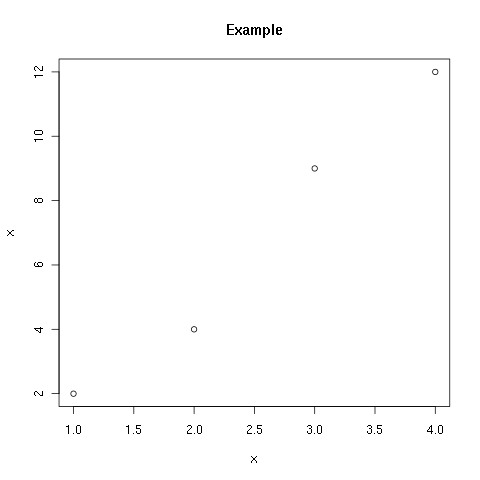
\includegraphics[width=3cm]{img/simpleCorrelationExample}

    \column{.3\textwidth}

    \only<2->
    {
      \begin{eqnarray*}
        \bar{x} & = & 2.5 \\
        \bar{y} & = & 6.75
      \end{eqnarray*}
    }

    \vfill

  \end{columns}

  \only<3->
  {
    \begin{eqnarray*}
      s_{xx} & = & \lp 1-2.5\rp^2 + \lp 2 - 2.5 \rp^2 + \lp 3 - 2.5 \rp^2 + \lp 4 - 2.5 \rp^2 \\
            & = & 5, \\
      s_{yy} & = & \lp 2-6.75\rp^2 + \lp 4 - 6.75 \rp^2 + \lp 9 - 6.75 \rp^2 + \lp 12 - 6.75 \rp^2 \\
            & = & 62.75, \\
      s_{xy} & = & \lp 1-2.5\rp\lp 2-6.75\rp + \lp 2 - 2.5 \rp\lp 4 - 6.75 \rp + \\
            &   & \lp 3 - 2.5 \rp\lp 9 - 6.75 \rp + \lp 4 - 2.5 \rp\lp 12 - 6.75 \rp \\
            & = & 17.5
    \end{eqnarray*}
  } 

  \only<4->
  {
    \vspace*{-2em}
    \begin{eqnarray*}
      r & = & \frac{17.5}{\sqrt{5\cdot 62.75}}, \\
        & \approx & 0.988
    \end{eqnarray*}
  }


\end{frame}



\begin{frame}{Correlation}

  \hspace*{-3em}
  \begin{tabular}{rrr}
    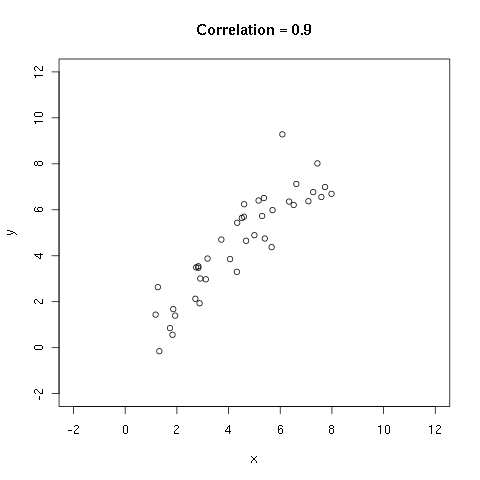
\includegraphics[height=4cm]{img/correlation09} & 
    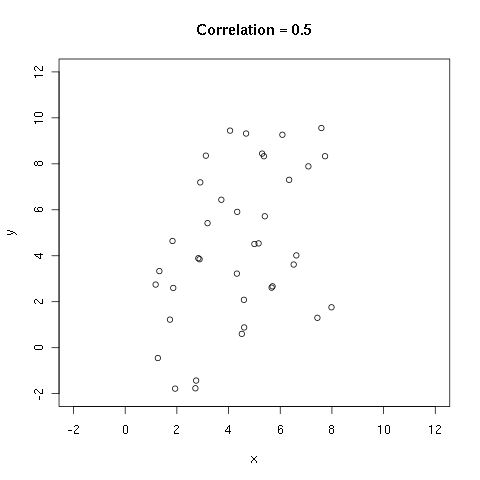
\includegraphics[height=4cm]{img/correlation05} &
    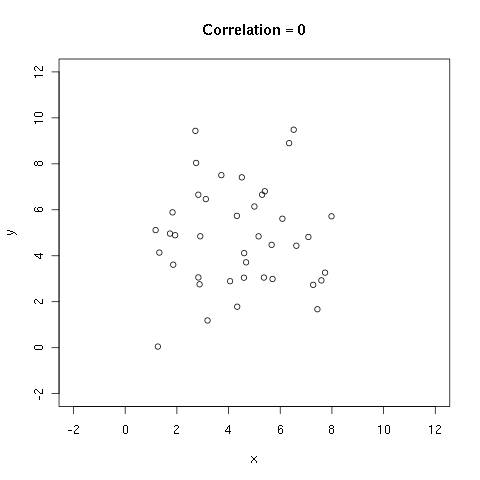
\includegraphics[height=4cm]{img/correlation0} \\
    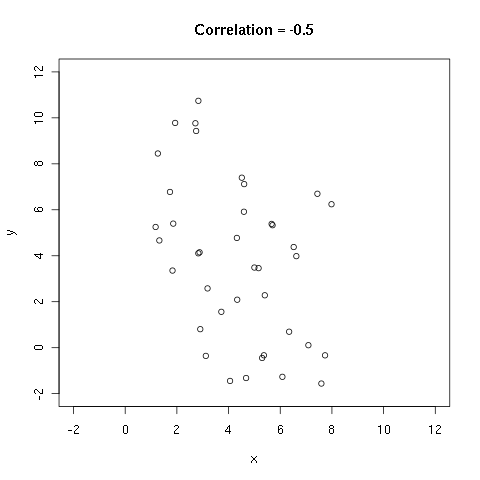
\includegraphics[height=4cm]{img/correlation-05} &
    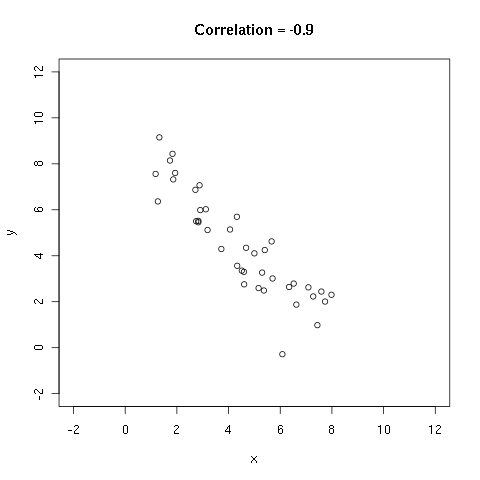
\includegraphics[height=4cm]{img/correlation-09}
  \end{tabular}


\end{frame}

\begin{frame}{Be Careful!}

  \begin{block}{Correlation}
    The value of $r$ tells you whether or not the general relationship
    is positive or negative and how closely it follows a linear
    relationship. It says nothing about the magnitude of the relationship!
  \end{block}
  
\end{frame}



% LocalWords:  Clarkson pausesection hideallsubsections Bivariate
